\structure{ОСНОВНАЯ~ЧАСТЬ}

\section{Структура алгоритма}

\begin{figure}
    \centering
    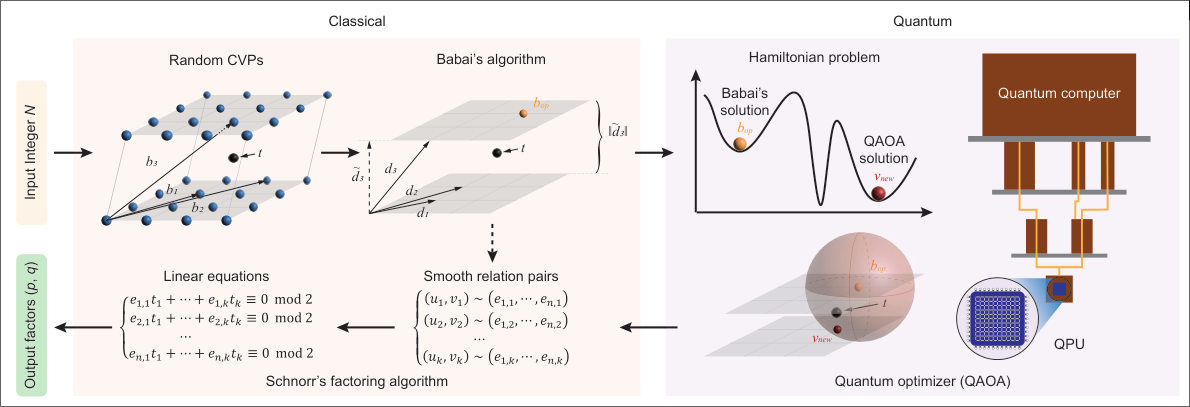
\includegraphics[scale=0.4]{inc/fig_01.png}
    \caption{
        Порядок работы квантового алгоритма факторизации целых чисел с
        сублинейными ресурсами (SQIF). Алгоритм использует гибридную
        «классическую+квантовую» структуру, в которой квантовый оптимизатор
        QAOA применяется для оптимизации классического алгоритма факторизации
        Шнорра. Сначала задача предварительно обрабатывается как задача
        ближайшего вектора (CVP) на решётке. Затем квантовый компьютер
        работает в качестве оптимизатора, уточняя классические векторы,
        полученные алгоритмом Бабая; на этом этапе находится решение CVP
        более высокого качества (то есть более близкое). Оптимизированные
        результаты передаются обратно в процедуру алгоритма Шнорра. После
        пост‑обработки в конце выводятся множители $p$ и $q$
    }
    \label{fig:fig01}
\end{figure}

Порядок работы квантового алгоритма факторизации целых чисел с сублинейными
ресурсами (SQIF) представлен на рис. \ref{fig:fig01}, который, по существу,
представляет собой гибридную «классическую+квантовую» структуру. Основная идея
состоит в использовании квантового оптимизатора QAOA для оптимизации самой
ресурсоёмкой части алгоритма Шнорра, что, в результате, повышает общую
эффективность процесса факторизации. Как показано на левой панели рис.
\ref{fig:fig01}, алгоритм Шнорра включает два существенных шага: поиск
достаточного количества пар гладких отношений (для краткости, sr‑пары) и
решение полученной системы линейных уравнений. Как правило, поиск sr‑пар
является самой важной и трудоёмкой частью алгоритма, тогда как решение системы
уравнений может быть выполнено за полиномиальное время. В алгоритме Шнорра
\cite{cite_31} задача sr‑пар преобразуется в задачу ближайшего вектора (CVP) на
решётке и решается посредством алгоритмов редукции базиса решётки, таких как
алгоритм Бабая \cite{cite_32}. Поскольку CVP является известной NP‑трудной
задачей \cite{cite_33}, мы можем рассчитывать только на приближённое, а не
точное решение CVP за полиномиальное или другое приемлемое время. Вероятность
получения sr‑пары пропорциональна качеству решения CVP \cite{cite_29}. То есть
чем ближе вектор‑решение CVP, тем эффективнее поиск sr‑пар. Исходя из
изложенного, мы предлагаем схему, в которой QAOA дополнительно оптимизирует
решение CVP, полученное алгоритмом Бабая. Полный процесс алгоритма SQIF
представлен в подробных примерах в \cite{cite_31}. В дальнейшем мы
сосредоточимся на квантовых этапах алгоритма.

Мы объединяем алгоритм Бабая с QAOA для решения CVP на решётке. Пусть дана
решётка $\Lambda$ с набором базиса $B=[b_1,\ldots,b_n]\in {R}^{(n+1)\times n}$
и целевой вектор ${t}\in{R}^{n+1}$. Алгоритм Бабая находит вектор
${b}_{{op}}\in\Lambda$, приближённо ближайший к ${t}$, в два шага. Сначала
выполняется LLL‑редукция с параметром~$\delta$ для заданного базиса~$B$. В
результате получаем LLL‑редуцированный базис $D=[d_1,\ldots,d_n]$ и
соответствующий ортогональный базис Грама–Шмидта
$\widetilde{D}=[\widetilde{d}_1,\ldots,\widetilde{d}_n]$. Второй шаг —
«уменьшение размера» целевого вектора ${t}$ с использованием
LLL‑редуцированного базиса. Так получаем приближённый ближайший вектор

\begin{equation}
    {b}_{{op}}
    = \bigl(b^{1}_{{op}},\ldots,b^{\,n+1}_{{op}}\bigr)^{\prime}
    = \sum_{i=1}^{n} c_{i}\,d_{i},
\end{equation}

где коэффициент $c_i=\lceil\mu_i\rfloor=
\left\lceil\langle{d},\widetilde{d}_i\rangle/
\langle\widetilde{d}_i,\widetilde{d}_i\rangle\right\rfloor$ получается
округлением к ближайшему целому коэффициента Грама–Шмидта~$\mu_i$. Здесь
следует отметить, что функция округления к ближайшему значению выполняет лишь
одно приближение за раз. Фактически, если значения двух функций округления
можно учесть одновременно, удаётся получить решение более высокого качества
\cite{cite_31}. Однако этот процесс экспоненциально увеличивает объём
классических операций, что неприемлемо для классического компьютера. Мы
применяем идею квантовых вычислений, используя суперпозицию кубитов для
одновременного кодирования значений коэффициентов, полученных двумя функциями
округления. Затем мы формулируем задачу оптимизации, основываясь на евклидовом
расстоянии между новым вектором решётки и целевым вектором. Подробности
построения приведены ниже.

Пусть $v_{new}$ — новый вектор, полученный случайным выбором $x_i\in\{0,\pm1\}$
на коэффициенте $c_i$, удовлетворяющий

\begin{equation}
    v_{new}
    \;=\;
    \sum_{i=1}^{n} (c_i + x_i)\,d_i
    \;=\;
    \sum_{i=1}^{n} x_i\,d_i + b_{op}.
\end{equation}

Мы определяем функцию потерь задачи оптимизации следующим образом

\begin{equation}
    F(x_{1},\ldots,x_{n})
    \;=\;
    \bigl\lVert t - v_{new} \bigr\rVert^{2}
    \;=\;
    \Bigl\lVert\,
        t - \sum_{i=1}^{n} x_i\,d_i - b_{op}
    \Bigr\rVert^{2}.
\end{equation}

Значение функции $\lVert t-v_{new}\rVert^{2}$ представляет собой квадрат
евклидова расстояния от нового вектора до целевого вектора. Чем меньше значение
функции потерь, тем ближе новый вектор к целевому вектору $t$ и тем выше
качество решения. Когда все переменные $x_{i,i=1,\ldots,n}$ принимают нулевые
значения, получаем оптимальное решение, выдаваемое алгоритмом Бабая.

Отображая переменную $x_i$ на операторы Паули‑$Z$, можно построить гамильтониан
задачи, соответствующий уравнению (3), в виде

\begin{equation}
    H_{C}
    \;=\;
    \Bigl\lVert
        t - \sum_{i=1}^{n} \hat{x}_{i}\,d_{i} - b_{op}
    \Bigr\rVert^{2}
    \;=\;
    \sum_{j=1}^{\,n+1}
    \Bigl|
    t_{j}
    - \sum_{i=1}^{n} \hat{x}_{i}\,d_{i,j}
    - b_{op}^{\,j}
    \Bigr|^{2}.
\end{equation}

где $\hat{x}_i$ — квантовый оператор, сопоставленный базису Паули‑$Z$ согласно
правилам однокубитного кодирования (см.~\cite{cite_31}).

В таком случае число кубитов, необходимых для квантовой процедуры оптимизации
алгоритма Бабая, равно размерности решётки. Согласно анализу из \cite{cite_31},
эта размерность удовлетворяет $n\sim 2c\log N/\log\log N$, где $c$ — параметр
решётки, близкий к 1. Следовательно, чтобы факторизовать $m$‑битное целое
число $N$, наш алгоритм требует $O(m/\log m)$ кубитов — сублинейную величину по
$m$, в то время как алгоритм Шора нуждается в $O(m)$ кубитах \cite{cite_13}, а
метод таблицы произведений — в $O(m^{2})$ кубитах \cite{cite_25}. Тем самым наш
алгоритм является самым экономичным по числу кубитов на сегодняшний день и
первым универсальным квантовым алгоритмом факторизации с сублинейными
квантовыми ресурсами.
